\section{Isotropic\_Sqw: A general $S(q,\omega)$ coherent and incoherent scatterer}
\label{s:isotropic-sqw}
\index{Samples!Coherent and incoherent isotropic scatterer}
\index{Coherent and incoherent isotropic scatterer}
\index{Inelastic scattering}
\index{Sample environments}
\index{Concentric components}
\index{Multiple scattering}

\component{Isotropic\_Sqw}{V. Hugouvieux, E. Farhi}{Sqw$\_{coh}$, $\sigma_{coh}$, Sqw$\_{inc}$, $\sigma_{inc}, V_\rho, \sigma_{abs}, T$,$x_{width},y_{height},z_{depth},r$, thickness}{$q_{min}, q_{max}, \omega_{min}, \omega_{max}, d\phi$, order}{validated (Vanadium, l-Rb, PowderN more accurate for powders) }

\begin{figure}
  \begin{center}
    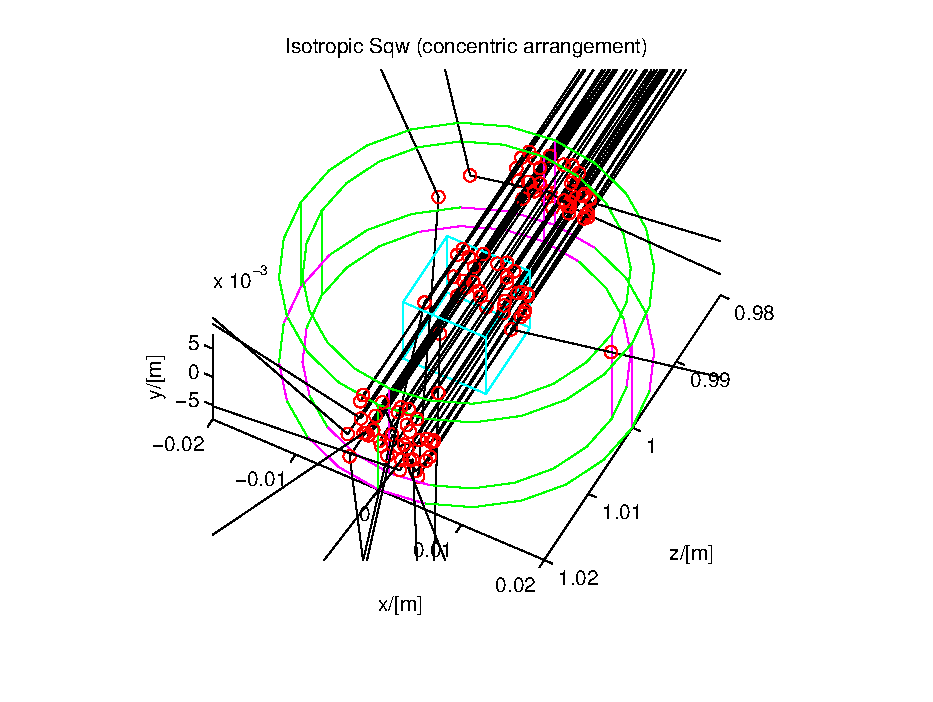
\includegraphics[width=0.9\textwidth]{figures/sqw}
  \end{center}
\caption{An $l-^4$He sample in a cryostat, simulated with the Isotropic\_Sqw component in concentric geometry.}
\label{f:isotropic-sqw}
\end{figure}

The sample component \emph{Isotropic\_Sqw} has been developed in order to simulate neutron scattering from any isotropic material such as liquids, glasses (amorphous systems), polymers and powders (currently, mono-crystals cannot be handled).
The component treats coherent and incoherent neutron scattering and may be used to model most materials, including sample environments with concentric geometries.
The structure and dynamics of isotropic samples can be characterised by the dynamic structure factor $S(q,\omega)$, which determines the interaction between neutrons and the sample and therefore can be used as a probability distribution of $\omega$-energy and $q$-momentum transfers. It handles coherent and incoherent processes, both for elastic and inelastic interactions.
The main input for the component is $S(q,\omega)$ tables, or powder structure files.

Usage examples of this component can be found in the \\
\verb+Neutron site/tests/Test_Isotropic_Sqw+, the \\
\verb+Neutron site/ILL/ILL_H15_IN6+ and the \verb+ILL_TOF_Env+ instruments from the \verb+mcgui+.

\subsection{Neutron interaction with matter - overview}

When a neutron enters a material, according to usual models, it 'sees' atoms as disks with a surface equal to the total cross section of the material $\sigma_{tot}$. The latter includes absorption, coherent and incoherent contributions, which all depend on the incoming neutron energy.
The transmission probability follows an exponential decay law accounting for the total cross section.

For the neutron which is not transmitted, we select a scattering position along the path, taking into account the secondary extinction and absorption probability. In this process, the neutron is considered to be a particle or an attenuated wave.

Once a scattering position has been assigned, the neutron interacts with a material excitation. Here we turn to the wave description of the neutron, which interacts with the whole sample volume. The distribution of excitations, which determines their relative intensity in the scattered beam, is simply the dynamic structure factor - or scattering law - $S(q,\omega)$. We shall build probability distributions from the scattering law in order to improve the efficiency of the method by favoring the $(q,\omega)$ choice towards high $S(q,\omega)$ regions.

The neutron leaves the scattering point when a suitable $(q, \omega)$ choice has been found to satisfy the conservation laws. The method is iterated until the neutron leaves the volume of the material, therefore allowing multiple scattering contributions, which will be considered in more details below.

No experimental method makes it possible to accurately measure the multiple scattering contribution, even though it can become significant at low $q$ transfers (below the first diffraction maximum), where the single scattering coherent signal is weak in most materials. This is why attemps have been made to reduce the multiple scattering contribution by partitioning the sample with absorbing layers. However, this is not always applicable thus makiong the simulation approach very valuable.

The method presented here for handling neutron interaction with isotropic materials is similar in many respects to the earlier MSC \cite{msc}, Discus \cite{discus} and MSCAT \cite{mscat} methods, but the implementation presented here is part of a more general treatment of a sample in an instrument.

\subsection{Theoretical side}

\subsubsection{Pair correlation function $g(r)$ and Dynamic structure factor $S(q,\omega)$}

In the following, we consider an isotropic medium irradiated with a cold or thermal neutron beam. We ignore the possible thermal fission events and assume that the incoming neutron energy does not correspond to a Breit-Wigner resonance in the material. Furthermore, we do not take into account quantum effects in the material, nor refraction and primary extinction.

Following Squires \cite{squires}, the experimental counterpart of the scattering law $S(q,\omega)$ is the neutron double differential scattering cross section for both coherent and incoherent processes:
\begin{equation}\label{eq:d2sigma}
\frac{d^2\sigma}{d\Omega dE_f} = \frac{\sigma}{4\pi}\frac{k_f}{k_i} N S(q, \omega)
\end{equation}
which describes the amount of neutrons scattered per unit solid angle $d\Omega$ and per unit final energy $dE_f$. In this equation, $N=\rho V$ is the number of atoms in the scattering volume $V$ with atomic number density $\rho$, $E_f, E_i, k_f, k_i$ are the kinetic energy and wavevectors of final and initial states respectively, $\sigma$ is the bound atom scattering cross-section, $\Omega$ is the solid angle and $q,\omega$ are the wave-vector and energy transfer at the sample. In practice, the double differential cross section is a linear combinaison of the coherent and incoherent parts as:
\begin{equation}
\label{eq:S=coh+inc}
\sigma S(q,\omega) = \sigma_{coh} S_{coh}(q,\omega) + \sigma_{inc} S_{inc}(q,\omega)
\end{equation}
where the subscripts $coh$ and $inc$ stand for the coherent and incoherent contributions respectively.

We define its norm on a selected $q$ range:
\begin{equation}
|S| = \iint S(q,\omega) dq d\omega .
\end{equation}
The norm $\lim_{q \rightarrow \infty} |S| \simeq q$ for large $q$ values, and can only be defined on a restricted $q$ range.

Some easily measureable coherent quantities in a liquid are the \emph{static pair correlation function} $g(r)$ and the \emph{structure factor} $S(q)$, defined as:
\begin{eqnarray}
\rho g(\vec{r}) &=& \frac{1}{N} \sum_{i=1}^N \sum_{j \neq i} \langle \delta(\vec{r}+\vec{r}_i-\vec{r}_j) \rangle \\
S(\vec{q}) &=&\int S(\vec q,\omega) d\omega \label{eq:sq} \\
           &=&1 + \rho \int_V [g(\vec{r})-1] e^{i\vec{q}.\vec{r}} d\vec{r} \\
           &=&1 + \rho \int_{0}^{\infty} [g(r)-1] \frac{\sin(qr)}{qr} 4 \pi r^2 dr {\rm\ in\ isotropic\ materials.}
\end{eqnarray}
The latter expression, in isotropic materials, may be Fourier transformed as:
\begin{equation}
\label{eq:gr-sq}
g(r)-1 =\frac{1}{2\pi^2 \rho} \int_0^\infty q^2 [S(q) -1] \frac{sin(qr)}{qr} dq
\end{equation}
Both $g(r)$ and $S(q)$ converge to unity for large $r$ and $q$ values respectively, and they are representative of the atoms spatial distribution. In a liquid $\lim_{q \rightarrow 0} S(q) = \rho k_B T \chi_T$ where $\chi_T=(\frac{\partial \rho}{\partial P})_{V,T}$ is the compressibility \cite{Egelstaff67,fischer05}. In perfect gases, $S(q) = 1$ for all $q$. These quantities are obtained experimentally from diffractometers.
In principle, $S_{inc}(q) = 1$ in all materials, but a $q$ dependence is rather usual, partly due to the Debye-Waller factor $e^{-q^2 \langle u^2 \rangle}$. Anyway, $S_{inc}(q)$ converges to unity at high $q$.

The static pair correlation function $g(r)$ is the probability to find a neighbouring atom at a given distance (unitless). Since $g(0) = 0$, Eq. (\ref{eq:gr-sq}) provides a useful normalisation sum-rule for coherent $S(q)$:
\begin{equation}
\label{eq:sq-nomr1}
\int_0^\infty q^2 [S(q) - 1] dq = -2\pi^2\rho {\rm\ for\ coherent\ contribution.}
\end{equation}
This means that the integrated oscillations (around 1) of $S_{coh}(q)$ are directly related to the density of the material $\rho$.
In practice, the function $S(q)$ is often known on a restricted range $q \in [0, q_{max} ]$, due to either limitations in the sample molecular dynamics simulation, or the measurement itself.
In first approximation we consider that Eq. (\ref{eq:sq-nomr1}) can be applied in this range, i.e. we neglect the large $q$ contributions provided $S(q)-1$ converges faster than $1/q^2$. This is usually true after 2-3 oscillations of $S(q)$ in liquids.
Then, in isotropic liquid-like materials, Eq. (\ref{eq:sq-nomr1}) provides a normalisation sum-rule for $S$.

\subsection{Theoretical side - scattering in the sample}

The Eq. \ref{eq:d2sigma} controls the scattering in the whole sample volume.
Its implementation in a propagative Monte Carlo neutron code such as \emph{McStas} can be summarised as follows:
\begin{enumerate}
{\item Compute the propagation path length in the material by geometrical intersections between the neutron trajectory and the sample volume.}
{\item Evaluate the total cross section from the integration of the scattering law over the accessible dynamical range (Section \ref{s:inter-proba}).}
{\item Use the total cross section to determine the probability of interaction for each neutron along the path length, and select a scattering position.}
{\item Weight neutron interaction with the absorption probability and select the type of interaction (coherent or incoherent).}
{\item Select the wave vector and energy transfer from the dynamic structure factor $S(q,\omega)$ used as a probability distribution (Section \ref{s:choose-qw}). Apply the detailed balance.}
{\item Check whether selection rules can be solved (Section \ref{s:rules-qw}). If they cannot, repeat (5).}
\end{enumerate}
This procedure is iterated until the neutron leaves the sample. We shall now detail the key steps of this implementation.

\subsubsection{Evaluating the cross sections and interaction probability}
\label{s:inter-proba}

Following Sears \cite{Sears75}, the total scattering cross section for incoming neutrons with initial energy $E_i$ is
\begin{equation}
\label{eq:iisigma}
\sigma_s(E_i) = \iint \frac{d^2 \sigma}{d\Omega dE_f} d\Omega dE_f = \frac{N \sigma}{4\pi} \iint \frac{k_f}{k_i} S(q, \omega) d\Omega dE_f
\end{equation}
where the integration runs over the entire space and all final neutron energies.
As the dynamic structure factor is defined in the $q,\omega$ space, the integration requires a variable change. Using the momentum conservation law and the solid angle relation $\Omega=2\pi(1-cos \theta)$, were $\theta$ is the solid angle opening, we draw:
\begin{equation}
\label{eq:iqSqw}
\sigma_s(E_i) = N \iint \frac{\sigma S(q,\omega) q}{2 k_i^2} dq d\omega.
\end{equation}
This integration runs over the whole accessible $q,\omega$ dynamical range for each incoming neutron.
In practice, the knowledge of the dynamic structure factor is defined over a limited area with $q \in [q_{min}, q_{max}]$ and $\omega \in [\omega_{min}, \omega_{max}]$ which is constrained by the method for obtaining $S(q,\omega)$, i.e. from previous experiments, molecular dynamics simulations, and analytical models. It is desirable that this area be as large as possible, starting from 0 for both ranges. If we use $\omega_{min} \rightarrow 0$, $q_{min} \rightarrow 0$, $\omega_{max} > 4E_i$ and $q_{max} > 2k_i$, we completely describe all scattering processes for incoming neutrons with wavevector $k_i$ \cite{msc}.

This means that in order to correctly estimate the total intensity and multiple scattering, the knowledge of $S(q,\omega)$ must be wider (at least twice in $q$, as stated previously) than the measurable range in the corresponding experiment.
As a side effect, a self consistent iterative method for finding the true scattering law from the measurement itself is not theorically feasible, except for providing crude approximations.
However, that measured dynamic structure factor may be used to estimate the multiple scattering for a further measurement using longer wavelength neutrons.
In that case, extrapolating the scattering law beyond the accessible measurement ranges might improve substantially the accuracy of the method, but this discussion is beyond the scope of this paper.

Consequently, limiting the $q$ integration in Eq. \ref{eq:iqSqw} to the maximum momentum transfer for elastic processes $2 k_i$, we write the total scattering cross section as
\begin{equation}
\label{eq:iqSq}
\sigma_s(E_i) \simeq \frac{N}{2 k_i^2} \int_0^{2k_i} q \sigma S(q) dq.
\end{equation}
Using Eq. \ref{eq:S=coh+inc}, it is possible to define similar expressions for the coherent and incoherent terms $\sigma_{coh}(E_i)$ and $\sigma_{inc}(E_i)$ respectively. These integrated cross sections are usually quite different from the tabulated values \cite{ILLblue} since the latter are bound scattering cross sections.

Except for a few materials with absorption resonances in the cold-thermal energy range, the absorption cross section for an incoming neutron of velocity $v_i=\sqrt{2E_i/m}$, where $m$ is the neutron mass, is computed as
$\sigma_{abs}(E_i) = \sigma_{abs}^{{\rm 2200}}\frac{2200 m/s}{\sqrt{2E_i/m}}$, where $\sigma_{abs}^{{\rm 2200}}$ is obtained from the literature \cite{ILLblue}.

We now determine the total cross section accounting for both scattering and absorption
\begin{equation}
\sigma_{tot}(E_i) = \sigma_{abs}(E_i) + \sigma_s(Ei).
\end{equation}
The neutron trajectory intersection with the sample geometry provides the total path length in the sample $d_{exit}$ to the exit.
Defining the linear attenuation $\mu(E_i) = \rho\sigma_{tot}(E_i)$, the probability that the neutron event is transmitted along path $d_{exit}$ is $e^{-\mu(E_i) d_{exit}}$.

If the neutron event is transmitted, it leaves the sample. In previous Monte Carlo codes such as DISCUSS \cite{discus}, MSC \cite{msc} and MSCAT \cite{mscat}, each neutron event is forced to scatter to the detector area in order to improve the sample scattering simulation statistics and reduce the computing time. The corresponding instrument model is limited to a neutron event source, a sample and a detector. It is equaly possible in the current implementation to 'force' neutron events to scatter by applying a correction factor $\pi_0=1-e^{-\mu(E_i) d_{exit}}$ to the neutron statistical weight. However, the \emph{McStas} instrument model is often build from a large sequence of components. Eventhough the instrument description starts as well with a neutron event source, more than one sample may be encountered in the course of the neutron propagation and multiple detectors may be positioned anywhere in space, as well as other instrument components (e.g. neutron optics). This implies that neutron events scattered from a sample volume should not focus to a single area.  Indeed, transmitted events may reach other scattering materials and it is not desirable to force all neutron events to scatter. The correction factor $\pi_0$ is then not applied, and neutron events can be transmitted through the sample volume. The simulation efficiency for the scattering then drops significantly, but enables to model much more complex arrangements such as concentric sample environments, magnets and monochromator mechanical parts, and neutron filters.

If the neutron is not transmitted, the neutron statistical weight is multiplied by a factor
\begin{equation}
\pi_1 = \frac{\sigma_s(E_i)}{\sigma_{tot}(E_i)}
\end{equation}
to account for the fraction of absorbed neutrons along the path, and we may in the following treat the event as a scattering event.
Additionally, the type of interaction (coherent or incoherent) is chosen randomly with fractions $\sigma_{coh}(E_i)$ and $\sigma_{inc}(E_i)$.

The position of the neutron scattering event along the neutron trajectory length $d_{exit}$ is determined by \cite{Mildner77,discus}
\begin{equation}
d_{s} = -\frac{1}{\mu(E_i)} \ln(1 - \xi[1 -e^{-\mu(E_i) d_{exit}}])
\end{equation}
where $\xi$ is a random number in [0,1]. This expression takes into account secondary extinction, originating from the decrease of the beam intensity through the sample (self shielding).

\subsubsection{Choosing the $q$ and $\omega$ transfer from $S(q, \omega)$ }
\label{s:choose-qw}

The choice of the $(q, \omega)$ wavevector-energy transfer pair could be done randomly, as in the first event of the second order scattering evaluation in DISCUS \cite{discus}, but it is somewhat inefficient except for materials showing a broad quasi-elastic signal. As the scattering originates from structural peaks and excitations in the material $S(q, \omega)$, it is usual \cite{mscat} to adopt an importance sampling scheme by focusing the $(q, \omega)$ choice to areas where the intensity of $S(q, \omega)$ is high. In practice, this means that the neutron event should scatter preferably on e.g. Bragg peaks, quasielastic contribution and phonons.

The main idea to implement the scattering from $S(q, \omega)$ is to cast two consecutive Monte Carlo choices, using probability distribution built from the dynamic structure factor.
We define first the probability $P_{\omega}(\omega)$ as the \emph{unweighted} fraction of modes whose energy lies between $\omega$ and $\omega+d\omega$
\begin{equation}
P_{\omega}(\omega) d\omega = \frac{\int_0^{q_{max}} q S(q,\omega) dq}{|S|},
\end{equation}
where $|S| = \iint S(q,\omega) dq d\omega$ is the norm of $S(q,\omega)$ in the available dynamical range $q \in [q_{min}, q_{max}]$ and $\omega \in [\omega_{min}, \omega_{max}]$.
The probability $P_{\omega}(\omega)$ is normalised to unity, $\int P_{\omega}(\omega) d\omega = 1$, and is a probability distribution of mode energies in the material. We then choose randomly an energy transfer $\omega$ from this distribution.

Similarly, in order to focus the wavevector transfer choice, we define the probability distribution of wavevector $P_q(q\mid\omega)$ for the selected energy transfer lying between $\omega$ and $\omega+d\omega$
\begin{equation}
P_q(q\mid\omega) = \frac{q S(q, \omega)}{S(q)},
\end{equation}
from which we choose randomly a wavevector transfer $q$, knowing the energy transfer $\omega$.
These two probability distributions extracted from $S(q,\omega)$ are shown in Fig. \ref{f:isotropic-sqw-proba}, for a model $S(q,\omega)$ function built from the {\it l}-$^4$He elementary excitation (Data from Donnelly).

\begin{figure}
  \begin{center}
    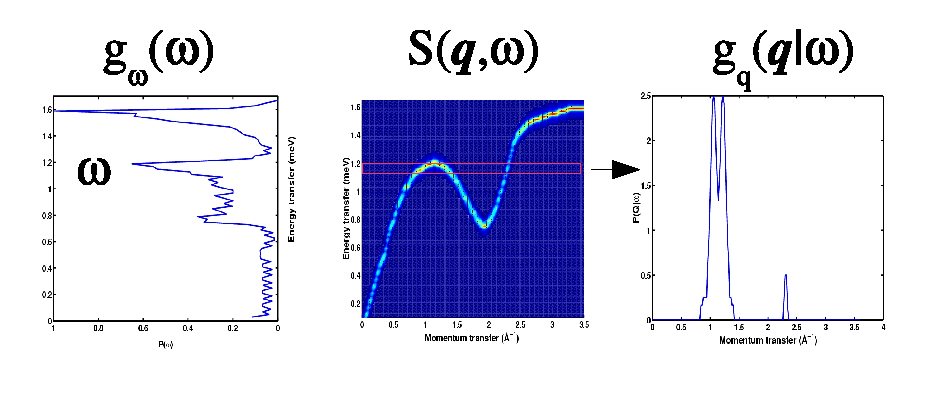
\includegraphics[width=0.9\textwidth]{figures/Sqw_sampling}
  \end{center}
\caption{\emph{Centre}: Model of dynamic structure factor $S(q,\omega)$ for l-$^4$He ; \emph{left}: probability distribution $g_\omega$ (horizontal axis) of energy transfers (vertical axis, density of states) ; \emph{right} : probability distribution $g_q(\omega)$ (vertical axis) of momentum transfers (horizontal axis) for a given energy transfer $\hbar \omega \sim 1.1$ meV.}
\label{f:isotropic-sqw-proba}
\end{figure}

Then a selection between energy gain and loss is performed with the detailed balance ratio $e^{-\hbar \omega / k_B T}$. In the case of Stokes processes, the neutron can not loose more than its own energy to the sample dynamics, so that $\hbar \omega < E_i$. This condition breaks the symmetry between up-scattering and down-scattering.

\subsubsection{Solving selection rules and choosing the scattered wave vector}
\label{s:rules-qw}

The next step is to check that the conservation laws
\begin{eqnarray}
\hbar \omega &=& E_i - E_f = \frac{\hbar^2}{2m}(k_i^2 - k_f^2) \label{eq:sqw-w-transfer} \\
\vec q &=& \vec k_i - \vec k_f \label{eq:sqw-q-transfer}
\end{eqnarray}
can be satisfied. These conditions are closely related to the method for selecting the outgoing wave vector direction.

When the final wave vector has to be computed, the quantities $\vec{k}_i$, $\hbar \omega$ and $q = |\vec{q}|$ are known.
We solve the energy conservation law Eq. (\ref{eq:sqw-w-transfer}) and we select randomly $k_f$ as one of the two roots.

The scattering angle $\theta$ from the initial $k_i$ direction is determined from the momentum conservation law $cos(\theta) = (k_i^2 + k_f^2 - q^2)/(2k_i k_f)$, which defines a scattering cone. We then choose randomly a direction on the cone.

If the selection rules can not be verified (namely $|cos(\theta)| > 1$), a new $(q,\omega)$ random choice is performed (see Section \ref{s:choose-qw}).
It might appear inefficient to select the energy and momentum tranfers first and check the selection rules afterwards. However, in practice, the number of iterations to actually scatter on a high probability process and satisfy these rules is limited, usually below 10. Moreover, as these two steps are simple, the whole process requires a limited number of computer operations.

As mentioned in Section \ref{s:inter-proba}, previous multiple scattering estimation codes \cite{msc,mscat,discus} force the outgoing neutron event to come into the detector area and time window, thus improving dramatically the code efficiency. This choice sets the measurable energy and momentum transfers for the last scattering event in the sample, so that the choice of the scattering excitation actually requires a more complex sampling mechanism for the dynamic structure factor. As the present implementation makes no assumption on the simulated instrument part which is behind the sample, we can not apply this method. Consequently, the efficiency of the sample scattering code is certainly lower than previous codes, but on the other hand it does not depend on the type of instrument simulation. In particular, it may be used to model any material in the course of the neutron propagation along the instrument model (filters, mechanical parts, samples, shields, radiation protections).

Once the scattering probability and position, the energy and momentum transfers and the neutron momentum after scattering have all been defined, the whole process is iterated until the neutron is transmitted and exits the sample volume.

\subsubsection{Extension to powder elastic scattering}

In principle, the component can work in purely elastic mode if only the $\omega = 0$ column is available in $S$.
Anyway, in the diffractionists world, people do not usually define scattering with $S(q)$ (Eq. \ref{eq:sq}), but through the scattering vector $\boldsymbol{\tau}$, multiplicity $z(\tau)$ (for powders), and $|F^2|$ structure factors including Debye-Waller factors, as in Eq. \ref{eq:sigma_coh_el}.

When doing diffraction, and neglecting inelastic contribution as first approximation, we may integrate Eq. \ref{eq:d2sigma}, keeping $k_i = k_f$.
\begin{eqnarray}
\left(\frac{d\sigma}{d\Omega}\right)_{\rm coh.el.}(|q|) &=& \int_0^\infty \frac{d^2\sigma_{coh}}{d\Omega dE_f} dE_f = \frac{N \sigma_{coh}}{4\pi} S_{coh}(q) \\
& = & N\frac{(2\pi)^3}{V_0}\sum_{\boldsymbol{\tau}} \delta(\boldsymbol{\tau} - \boldsymbol{q})|F_{\boldsymbol{\tau}}|^2 {\rm\ from\ Eq.\ (\ref{eq:sigma_coh_el})}
\end{eqnarray}
with $V_0 = 1/\rho$ being the volume of a lattice unit cell. Then we come to the formal equivalence, in the powder case \cite{squires} (integration over Debye-Scherrer cones):
\begin{eqnarray}\label{eq:sq-F2}
S_{coh}(q) = \frac{\pi \rho}{2\sigma_{coh}} \frac{z(q)}{q^2} |F_q|^2 {\rm\ in\ a\ powder.}
\end{eqnarray}
for each lattice Bragg peak wave vector $q$.
The normalisation rule Eq. (\ref{eq:sq-nomr1}) can not usually be applied for powders, as the $S(q)$ is a set of Dirac peaks for which the $\int q^2 S(q) dq$ is difficult to compute, and $S(q)$ does not converge to unity for large $q$. Each $F^2$ Dirac contribution may be broaden when specifiying a diffraction peak width.

Of course, the component PowderN (see section \ref{powder}) can handle powder samples efficiently (faster, better accuracy), but does not take into account multiple scattering, nor secondary extinction (which is significant for materials with large absorption cross sections). On the other side, the current Isotropic\_Sqw component assumes a powder packing factor of 1 (massive sample). To change into a lower packing factor, use a lower powder density.

\subsubsection{Important remarks and limitations}

Since the choice of the interaction type, we know that the neutron \emph{must} scatter, with an appropriate $\vec k_f$ outgoing wave vector. If any of the choices in the method fails:
\begin{enumerate}
\item the two roots $k_f^+$ and $k_f^-$ are imaginary, which means that conservation laws can not be satisfied and for instance the selected energy transfer is higher than the incoming neutron energy
\item the radius of the target circle is imaginary, that is $|cos(\theta)| > 1$.
\end{enumerate}
then a new $(q, \omega)$ set is drawn, and the process is iterated until success or - at last - removal of the neutron event. These latter absorptions are then reported at the end of the simulation, as it never occurs in reality - neutrons that scatter do find a suitable $(q, \omega)$ set.\index{Removed neutron events}

The $S(q,\omega)$ data sets should be as wide a possible in $q$ and $\omega$ range, else scattering conditions will be limited by the reduced data set (specially multiple scattering estimates). On the other hand, when $q$ and $\omega$ ranges are too large, some Monte Carlo choices lead to scattering temptatives in non useful regions of $S$, which reduces dramatically the algorithm efficiency.

The best settings are:
\begin{enumerate}
\item to have the widest $q$ and $\omega$ range for $S(q,\omega)$ data sets,
\item to either set $wmax$ and $qmax$ to the maximum scatterable energy and wavevectors,
\item or alternatively request the automatic range optimisation by setting parameter \verb+auto_qw=1+. This is recommended, but may sometimes miss a few neutrons if the $q,\omega$ beam range has been guessed too small.
\end{enumerate}

Focusing the $q$ and $\omega$ range (e.g. with 'auto\_qw=1'), to the one being able to scatter the incoming beam, when using the component does improve significantly the speed of the computation. Additionally, if you restrict the scattering to the first order only (parameter 'order=1'), then you may specify the angular vertical extension $d\phi$ of the scattering area to gain optimised focusing. This option does not apply when handling multiple scattering (which emits in $4\pi$ many times before exiting the sample).

A bilinear interpolation for the $q,\omega$ determination is used to improve the accuracy on the scattered intensity, but it may be unactivated when setting parameter \verb+interpolate=0+. This will often result in a discrete $q,\omega$ sampling.

As indicated in the previous section, the Isotropic\_Sqw component is not as efficient as PowderN for powder single scattering, but handles scattering processes in a more accurate way (secondary extinction, multiple scattering).

\subsection{The implementation}

\begin{table}
  \begin{center}
  {\let\my=\\
    \begin{tabular}{|lr|p{0.6\textwidth}|}
    \hline
Parameter & type & meaning \\
    \hline
Sqw\_coh   & string              & Coherent scattering data file name. Use 0, NULL or "" to disable  \\
Sqw\_inc   & string              & Incoherent scattering data file name. Use 0, NULL or "" to scatter isotropically (Vanadium like)  \\
sigma\_coh & [barns]      & Coherent scattering cross-section. -1 to disable \\
sigma\_inc & [barns]      & Incoherent scattering cross-section. -1 to disable \\
sigma\_abs & [barns]      & Absorption cross-section. -1 to disable  \\
V\_rho     & [\AA$^{-3}$] & atomic number density. May also be specified with molar weight \emph{weight} in [g/mol] and material \emph{density} in [g/cm$^3$] \\
T          & [K]          & Temperature. 0 disables detailed balance \\
    \hline
xwidth   & [m] & \\
yheight  & [m] & dimensions of a box shaped geometry \\
zdepth   & [m] & \\
radius\_o & [m] & dimensions of a cylinder shaped geometry  \\
radius\_i & [m] & sphere geometry if radius\_i=0  \\
thickness& [m] & thickness of hollow shape  \\
    \hline
auto\_qw  & boolean & Automatically optimise probability tables during simulation  \\
auto\_norm& scalar  & Normalize $S(q,\omega)$ when -1, use raw data when 0, multiply $S$ by given value when positive \\
%interpolate & boolean & Smooth $S(q,\omega)$ table (recommended) \\
order     & integer & Limit multiple scattering up to given order. 0 means all orders  \\
concentric& boolean & Enables to 'enter' inside concentric hollow geometries  \\
    \hline
    \end{tabular}
    \caption{Main Isotropic\_Sqw component parameters}
    \label{t:sqw-param}
  }
  \end{center}
\end{table}

\subsubsection{Geometry}

The geometry for the component may be box, cylinder and sphere shaped, either filled or hollow. Relevant parameters for this purpose are as follow:
\begin{itemize}
\item {\bf box}: dimensions are $x_{width} \times y_{height} \times z_{depth}$.
\item {\bf box, hollow}: \emph{idem}, and the side wall thickness is set with $thickness$.
\item {\bf cylinder}: dimensions are $r$ for the radius and $y_{height}$ for the height.
\item {\bf cylinder, hollow}: \emph{idem}, and hollow part is set with $thickness$.
\item {\bf sphere}: dimension is $r$ for the radius.
\item {\bf sphere, hollow}: \emph{idem}, and hollow part is set with $thickness$.
\end{itemize}
The AT position corresponds to the centre of the sample.

Hollow shapes are particularly useful to model complex sample environments. Refer to the dedicated section below for more details on this topic.

\subsubsection{Dynamical structure factor}

The material behaviour is specified through the total scattering cross-sections $\sigma_{coh}$, $\sigma_{inc}$, $\sigma_{abs}$, and the $S(q, \omega)$ data files.

If you are lucky enough to have access to separated coherent and incoherent contributions (e.g. from material simulation), simply set Sqw\_coh and Sqw\_inc parameter to the files names. If on the other hand you have access to a global data set containing incoherent scattering as well (e.g. the result of a previous experiment), use Sqw\_coh parameter, set the $\sigma_{coh}$ parameter to the sum of both contributions $\sigma_{coh}+\sigma_{inc}$, and set $\sigma_{inc}=-1$. This way we only use one of the two implemented  scattering channels. Such global data sets may originate from previous experiments, as far as you have applied all known corrections (multiple scattering, geometry, ...).

In any case, the accuracy of the $S(q, \omega)$ data limits the $q$ and $\omega$ resolution of the simulation, eventhough a bilinear interpolation is performed in order to smooth binning. The sampling of data files should then be as thin as possible.

If the Sqw\_inc parameter is left unset but the $\sigma_{inc}$ is \emph{not} zero, an isotropic incoherent elastic scattering is used, just like the V\_sample component (see section \ref{s:v_sample}).

Anyway, as explained below, it is also possible to simulate the elastic scattering from a powder file (see below).

\subsubsection{File formats: $S(q,\omega)$ inelastic scattering}

The format of the data files is free text, consisting of three numerical blocks, separated by empty lines or comments, in the following order
\begin{enumerate}
\item A vector of length $m$ containing wavevector $q$ values, in \AA$^{-1}$.
\item A vector of length $n$ containing energy $\omega$ values, in meV.
\item A matrix of size $m$ rows by $n$ columns, of $S(q, \omega)$ values, in meV$^{-1}$.
\end{enumerate}
Any line beginning with any character of \verb+#;/%+ is considered to be a comment, and lines which can not be read as vectors/matrices are ignored.

The file header may optionally contain parameter settings for the material, as comments, with keywords as in the following example:
\begin{lstlisting}
  #V_0         35   cell volume [Angs^3]
  #V_rho       0.07 atom number density [at/Angs^3]
  #sigma_abs   5    absorption cross section [barns]
  #sigma_inc   4.8  incoherent cross section [barns]
  #sigma_coh   1    coherent cross section  [barns]
  #Temperature 10   for detailed balance [K]
  #density     1    material density [g/cm^3]
  #weight      18   material molar weight [g/mol]
  #nb_atoms    6    number of atoms per unit cell
\end{lstlisting}
Some \verb+sqw+ data files are included in the \MCS distribution data directory, and they contain material parameter settings in their header, so that you may use:
\begin{lstlisting}
Isotropic_Sqw(<geometry parameters>, Sqw_coh="He4_liq_coh.sqw", T=4)
\end{lstlisting}

Example files are listed as \verb+*.sqw+ files in directory \verb+MCSTAS/data+. A table of $S(q,\omega)$ data files for a few liquids are listed in Table \ref{t:liquids-data} (page \pageref{t:liquids-data}).

\subsubsection{File formats: $S(q)$ liquids}

This file format provides a mean to import directly an $S(q)$ data set, when setting parameters:
\begin{lstlisting}
  powder_format=qSq
\end{lstlisting}
The 'Sqw\_coh' (or 'Sqw\_inc') file should contains a single numerical block, which column assignment is defaulted as $q$ and $S(q)$ being the first and second column respectively. This may be overridden from the file header with '\#column' keywords, as in the example:
\begin{lstlisting}
  #column_q  2
  #column_Sq 1
\end{lstlisting}
Such files can only handle elastic scattering.

\subsubsection{File formats: powder structures (LAZY, Fullprof, Crystallographica)}

Data files as used by the component PowderN may also be read. Data files of type \verb'lau' and \verb'laz' in the \MCS distribution data directory are self-documented in their header. They do not need any additional parameters to be used, as in the example:
\begin{lstlisting}
  Isotropic_Sqw(<geometry parameters>, Sqw_coh="Al.laz")
\end{lstlisting}
Other column-based file formats may also be imported e.g. with parameters such as:
\begin{lstlisting}
  powder_format=Crystallographica
  powder_format=Fullprof
  powder_Dd    =0
  powder_DW    =1
\end{lstlisting}
The last two parameters may as well be specified in the data file header with lines:
\begin{lstlisting}
  #Debye_Waller 1
  #Delta_d/d    1e-3
\end{lstlisting}
The powder description is then translated into $S(q)$ by using Eq. (\ref{eq:sq-F2}).
In this case, the density $\rho = n/V_0$ is the number of atoms in the inverse volume of the unit cell.

As the component builds an $S(q)$ from the powder structure description, the accuracy of the Isotropic\_Sqw component is limited by the binning during that conversion. This is usually enough to describe sample environments including powders (aluminium, copper, ...), but it is recommended to rather use PowderN for faster and accurate powder diffraction, eventthough this latter does not implement multiple scattering.

Such files can only handle elastic scattering. A list of common powder definition files is available in Table \ref{t:powders-data} (page \pageref{t:powders-data}).

\subsubsection{Concentric geometries, sample environment}
\index{Sample environments}

The component has been designed in a way which enables to describe complex imbricated set-ups, i.e. what you need to simulate sample environments. To do so, one has first to use hollow shapes, then keep in mind that each surrounding geometry should be first declared before the central position (usually the sample) with the \verb+concentric=1+ parameter, but also duplicated (with an other instance name) at a symmetric position with regards to the centre as in the example (shown in Fig. \ref{f:isotropic-sqw}):
\begin{lstlisting}
COMPONENT s_in=Isotropic_Sqw(
  thickness=0.001, radius=0.02, yheight=0.015,
  Sqw_coh="Al.laz", concentric=1)
AT (0,0,1) RELATIVE a

COMPONENT sample=Isotropic_Sqw(
  xwidth=0.01, yheight=0.01, zdepth=0.01,
  Sqw_coh="Rb_liq_coh.sqw")
AT (0,0,1) RELATIVE a

COMPONENT s_out=Isotropic_Sqw(
  thickness=0.001, radius=0.02, yheight=0.015,
  Sqw_coh="Al.laz")
AT (0,0,1) RELATIVE a
\end{lstlisting}
Central component may be of any type, not specifically an Isotropic\_Sqw instance. It could be for instance a Single\_crystal or a PowderN.
In principle, the number of surrounding shells is not restricted.
The only restriction is that neutrons that scatter (in $4\pi$) can not come back in the instrument description, so that some of the multiple scattering events are lost. Namely, in the previous example, neutrons scattered by the outer wall of the cryostat \verb+s_out+ can not come back to the sample or to the other cryostat wall \verb+s_in+. As these neutrons have usually few chances to reach the rest of the simulation, we expect that the approximation is fair.

\subsection{Validation}
For constant incoherent scattering mode, V\_sample, PowderN, Single\_crystal and Isotropic\_Sqw produce equivalent results, eventhough the two later are more accurate (geometry, multiple scattering). Execution times are equivalent.

Compared with the PowderN component, the $S(q)$ method is twice slower in computation time, and intensity is usually lower by typically 20 \% (depending on scattering cross sections), the difference arising from multiple scattering and secondary extinction (not handled in PowderN). The PowderN component is intrinsically more accurate in $q$ as each Bragg peak is handled separately as an exact Dirac peak, with optional $\Delta q$ spreading. In Isotropic\_Sqw, an approximated $S(q)$ table is built from the $F^2$ data, and is coarser. Still, differences in the diffraction pattern are limited.

The Isotropic\_Sqw component has been benchmarked against real experiment for liquid Rubidium (Copley, 1974) and liquid Cesium (Bodensteiner  and Dorner, 1989), and the agreement is excellent.

The \verb+Test_Isotropic_Sqw+ test/example instrument exists in the distribution for this component.



